\documentclass[twoside]{book}

% Packages required by doxygen
\usepackage{fixltx2e}
\usepackage{calc}
\usepackage{doxygen}
\usepackage[export]{adjustbox} % also loads graphicx
\usepackage{graphicx}
\usepackage[utf8]{inputenc}
\usepackage{makeidx}
\usepackage{multicol}
\usepackage{multirow}
\PassOptionsToPackage{warn}{textcomp}
\usepackage{textcomp}
\usepackage[nointegrals]{wasysym}
\usepackage[table]{xcolor}

% Font selection
\usepackage[T1]{fontenc}
\usepackage[scaled=.90]{helvet}
\usepackage{courier}
\usepackage{amssymb}
\usepackage{sectsty}
\renewcommand{\familydefault}{\sfdefault}
\allsectionsfont{%
  \fontseries{bc}\selectfont%
  \color{darkgray}%
}
\renewcommand{\DoxyLabelFont}{%
  \fontseries{bc}\selectfont%
  \color{darkgray}%
}
\newcommand{\+}{\discretionary{\mbox{\scriptsize$\hookleftarrow$}}{}{}}

% Page & text layout
\usepackage{geometry}
\geometry{%
  a4paper,%
  top=2.5cm,%
  bottom=2.5cm,%
  left=2.5cm,%
  right=2.5cm%
}
\tolerance=750
\hfuzz=15pt
\hbadness=750
\setlength{\emergencystretch}{15pt}
\setlength{\parindent}{0cm}
\setlength{\parskip}{3ex plus 2ex minus 2ex}
\makeatletter
\renewcommand{\paragraph}{%
  \@startsection{paragraph}{4}{0ex}{-1.0ex}{1.0ex}{%
    \normalfont\normalsize\bfseries\SS@parafont%
  }%
}
\renewcommand{\subparagraph}{%
  \@startsection{subparagraph}{5}{0ex}{-1.0ex}{1.0ex}{%
    \normalfont\normalsize\bfseries\SS@subparafont%
  }%
}
\makeatother

% Headers & footers
\usepackage{fancyhdr}
\pagestyle{fancyplain}
\fancyhead[LE]{\fancyplain{}{\bfseries\thepage}}
\fancyhead[CE]{\fancyplain{}{}}
\fancyhead[RE]{\fancyplain{}{\bfseries\leftmark}}
\fancyhead[LO]{\fancyplain{}{\bfseries\rightmark}}
\fancyhead[CO]{\fancyplain{}{}}
\fancyhead[RO]{\fancyplain{}{\bfseries\thepage}}
\fancyfoot[LE]{\fancyplain{}{}}
\fancyfoot[CE]{\fancyplain{}{}}
\fancyfoot[RE]{\fancyplain{}{\bfseries\scriptsize Generated by Doxygen }}
\fancyfoot[LO]{\fancyplain{}{\bfseries\scriptsize Generated by Doxygen }}
\fancyfoot[CO]{\fancyplain{}{}}
\fancyfoot[RO]{\fancyplain{}{}}
\renewcommand{\footrulewidth}{0.4pt}
\renewcommand{\chaptermark}[1]{%
  \markboth{#1}{}%
}
\renewcommand{\sectionmark}[1]{%
  \markright{\thesection\ #1}%
}

% Indices & bibliography
\usepackage{natbib}
\usepackage[titles]{tocloft}
\setcounter{tocdepth}{3}
\setcounter{secnumdepth}{5}
\makeindex

% Hyperlinks (required, but should be loaded last)
\usepackage{ifpdf}
\ifpdf
  \usepackage[pdftex,pagebackref=true]{hyperref}
\else
  \usepackage[ps2pdf,pagebackref=true]{hyperref}
\fi
\hypersetup{%
  colorlinks=true,%
  linkcolor=blue,%
  citecolor=blue,%
  unicode%
}

% Custom commands
\newcommand{\clearemptydoublepage}{%
  \newpage{\pagestyle{empty}\cleardoublepage}%
}

\usepackage{caption}
\captionsetup{labelsep=space,justification=centering,font={bf},singlelinecheck=off,skip=4pt,position=top}

%===== C O N T E N T S =====

\begin{document}

% Titlepage & ToC
\hypersetup{pageanchor=false,
             bookmarksnumbered=true,
             pdfencoding=unicode
            }
\pagenumbering{roman}
\begin{titlepage}
\vspace*{7cm}
\begin{center}%
{\Large B\+A\+R\+ES \\[1ex]\large 1.\+0 }\\
\vspace*{1cm}
{\large Generated by Doxygen 1.8.11}\\
\end{center}
\end{titlepage}
\clearemptydoublepage
\tableofcontents
\clearemptydoublepage
\pagenumbering{arabic}
\hypersetup{pageanchor=true}

%--- Begin generated contents ---
\chapter{B\+A\+R\+ES (Basic Arithmetic Expression Evaluator based on Stacks)}
\label{index}\hypertarget{index}{}\begin{DoxyAuthor}{Author}
Adelino Afonso Fernandes Avelino 

Irene Ginani Costa Pinheiro 
\end{DoxyAuthor}
\begin{DoxyDate}{Date}
Maio, 2016 
\end{DoxyDate}
\begin{DoxyVersion}{Version}
1.\+0 
\end{DoxyVersion}

\chapter{Projeto B\+A\+R\+ES}
\label{md_README}
\hypertarget{md_README}{}
Basic Arithmetic Expression Evaluator based on Stacks

\subsection*{Descrição}

O B\+A\+R\+ES (Basic A\+Rithmetic Expression Evaluator based on Stacks) e um avaliador de expressoes baseado em pilhas que recebe um conjunto de expressoes e verifica se as mesmas sao validas retornando o resultado da operacao, caso seja invalida o erro sera mostrado na coluna da espressao. Vale salientar que cada expressao deve estar em uma linha do arquivo para ser valida, quebras de linha na expressao torna-\/a invalida para calculos. Cada valor de expressao tem o tamanho de um inteiro, ou seja, deve estar entre -\/32767 e 32767. Abaixo segue uma tabela de operacoes suportadas pelo B\+A\+R\+ES.

\subsubsection*{Operadores Suportados}

\tabulinesep=1mm
\begin{longtabu} spread 0pt [c]{*3{|X[-1]}|}
\hline
\rowcolor{\tableheadbgcolor}\PBS\centering {\bf Simbolo }&{\bf Operacoes }&\PBS\centering {\bf Precedencia  }\\\cline{1-3}
\endfirsthead
\hline
\endfoot
\hline
\rowcolor{\tableheadbgcolor}\PBS\centering {\bf Simbolo }&{\bf Operacoes }&\PBS\centering {\bf Precedencia  }\\\cline{1-3}
\endhead
\PBS\centering \+\_\+\+\_\+ &Menos unario &\PBS\centering 1 \\\cline{1-3}
\PBS\centering \+\_\+\+\_\+$^\wedge$\+\_\+\+\_\+ &Exponenciacao &\PBS\centering 2 \\\cline{1-3}
\PBS\centering \+\_\+\+\_\+/\+\_\+\+\_\+ &Divisao &\PBS\centering 3 \\\cline{1-3}
\PBS\centering \+\_\+\+\_\+\+\_\+\+\_\+ &Modulo &\PBS\centering 3 \\\cline{1-3}
\PBS\centering \+\_\+\+\_\+$\ast$\+\_\+\+\_\+ &Multiplicacao &\PBS\centering 3 \\\cline{1-3}
\PBS\centering \+\_\+\+\_\+-\/\+\_\+\+\_\+ &Subtracao &\PBS\centering 4 \\\cline{1-3}
\PBS\centering \+\_\+\+\_\++\+\_\+\+\_\+ &Adicao &\PBS\centering 4 \\\cline{1-3}
\PBS\centering \+\_\+\+\_\+()\+\_\+\+\_\+ &Parenteses &\PBS\centering 5 \\\cline{1-3}
\end{longtabu}


\subsection*{Compilação}

g++ -\/std=c++11 -\/pedantic -\/I include/ \hyperlink{drive_8cpp}{src/drive.\+cpp} -\/o bin/exe

\subsection*{Execução}

Dentro da pasta B\+A\+R\+ES execute\+:

\$ ./bin/exe data/data.\+txt

\subsection*{Lista de erros que o programa trata}


\begin{DoxyEnumerate}
\item Numeric constant out of range\+: Um dos operandos da expressao esta fora da faixa permitida. Ex.\+: 1000000 − 2, coluna 1.
\item Ill-\/formed expression or missing term detected\+: Em alguma parte da expressao esta faltando um operando ou existe algum operando em formato errado. Ex.\+: 2+, coluna 3; ou 3 ∗ d, coluna 5.
\item Invalid operand\+: Existe um sımbolo correspondente a um operador que nao esta na lista de operadores validos. Ex.\+: 2 = 3, coluna 3; ou 2.\+3+4, coluna 2.
\item Extraneous symbol\+: Aparentemente o programa encontrou um sımbolo extra “perdido” na expressao. Ex.\+: 2 ∗ 3 4, coluna 7 ou (−3∗4)(10∗5), coluna 7.
\item Mismatch ’)’\+: Existem um parˆentese fechando sem ter um parentese abrindo correspondente. Ex.\+: )2−4, coluna 1; ou 2 − 4), coluna 6; ou 2) − 4. coluna 2.
\item Lost operator\+: Apareceu um operador sem seus operandos. 2 ∗∗ 3,coluna4;ou/5 ∗ 10,coluna 1.
\item Missing closing ‘)’ to match opening ‘)’ at\+: Esta faltando um parentese de fechamento ’)’ para um parentese de abertura ‘(’ correspondente. Ex.\+: ((2\%3) ∗ 8, coluna 1.
\item Division by zero!\+: Houve divisao cujo quociente e zero. Ex.\+: 3/(1 − 1); ou 10/(3 ∗ 3ˆ−2). Nestes casos nao e preciso informar a coluna.
\item Numeric overflow error!\+: Acontece quando uma operacao dentro da expressao ou a expressao inteira estoura o limite das constantes numericas definidos na Secao 1. Ex.\+: 20 ∗ 20000. Nestes casos nao e preciso informar a coluna.
\end{DoxyEnumerate}

\subsubsection*{Limitacoes}


\begin{DoxyItemize}
\item O programa não está tratando unário
\end{DoxyItemize}

\subsection*{Autores\+:}


\begin{DoxyItemize}
\item Adelino Afonso Fernandes Avelino -\/ \href{mailto:adelino-afonso@hotmail.com}{\tt adelino-\/afonso@hotmail.\+com}
\item Irene Ginani Costa Pinheiro -\/ \href{mailto:ireneginani@gmail.com}{\tt ireneginani@gmail.\+com} 
\end{DoxyItemize}
\chapter{Hierarchical Index}
\section{Class Hierarchy}
This inheritance list is sorted roughly, but not completely, alphabetically\+:\begin{DoxyCompactList}
\item \contentsline{section}{Abs\+Queue$<$ Object $>$}{\pageref{class_abs_queue}}{}
\begin{DoxyCompactList}
\item \contentsline{section}{Queue\+Ar$<$ Object $>$}{\pageref{class_queue_ar}}{}
\end{DoxyCompactList}
\item \contentsline{section}{Abs\+Queue$<$ std\+:\+:string $>$}{\pageref{class_abs_queue}}{}
\begin{DoxyCompactList}
\item \contentsline{section}{Queue\+Ar$<$ std\+:\+:string $>$}{\pageref{class_queue_ar}}{}
\end{DoxyCompactList}
\item \contentsline{section}{Abs\+Stack$<$ Object $>$}{\pageref{class_abs_stack}}{}
\begin{DoxyCompactList}
\item \contentsline{section}{Stack\+Ar$<$ Object $>$}{\pageref{class_stack_ar}}{}
\end{DoxyCompactList}
\item \contentsline{section}{conjuntura}{\pageref{classconjuntura}}{}
\end{DoxyCompactList}

\chapter{Class Index}
\section{Class List}
Here are the classes, structs, unions and interfaces with brief descriptions\+:\begin{DoxyCompactList}
\item\contentsline{section}{\hyperlink{class_abs_queue}{Abs\+Queue$<$ Object $>$} }{\pageref{class_abs_queue}}{}
\item\contentsline{section}{\hyperlink{class_abs_stack}{Abs\+Stack$<$ Object $>$} }{\pageref{class_abs_stack}}{}
\item\contentsline{section}{\hyperlink{classconjuntura}{conjuntura} \\*Classe conjuntura }{\pageref{classconjuntura}}{}
\item\contentsline{section}{\hyperlink{class_queue_ar}{Queue\+Ar$<$ Object $>$} \\*Classe \hyperlink{class_queue_ar}{Queue\+Ar} }{\pageref{class_queue_ar}}{}
\item\contentsline{section}{\hyperlink{class_stack_ar}{Stack\+Ar$<$ Object $>$} \\*Classe \hyperlink{class_stack_ar}{Stack\+Ar} }{\pageref{class_stack_ar}}{}
\end{DoxyCompactList}

\chapter{File Index}
\section{File List}
Here is a list of all documented files with brief descriptions\+:\begin{DoxyCompactList}
\item\contentsline{section}{include/{\bfseries Abs\+Queue.\+h} }{\pageref{_abs_queue_8h}}{}
\item\contentsline{section}{include/{\bfseries Abs\+Stack.\+h} }{\pageref{_abs_stack_8h}}{}
\item\contentsline{section}{include/\hyperlink{header_8h}{header.\+h} \\*Corpo da Classe Conjuntura }{\pageref{header_8h}}{}
\item\contentsline{section}{include/\hyperlink{header_8inl}{header.\+inl} \\*Implementação da Classe conjuntura }{\pageref{header_8inl}}{}
\item\contentsline{section}{include/\hyperlink{queuear_8h}{queuear.\+h} \\*Corpo da classe \hyperlink{class_queue_ar}{Queue\+Ar} }{\pageref{queuear_8h}}{}
\item\contentsline{section}{include/\hyperlink{queuear_8inl}{queuear.\+inl} \\*Implementação da classe \hyperlink{class_queue_ar}{Queue\+Ar} }{\pageref{queuear_8inl}}{}
\item\contentsline{section}{include/\hyperlink{stackar_8h}{stackar.\+h} \\*Corpo da classe \hyperlink{class_stack_ar}{Stack\+Ar} }{\pageref{stackar_8h}}{}
\item\contentsline{section}{include/\hyperlink{stackar_8inl}{stackar.\+inl} \\*Implementação da classe \hyperlink{class_stack_ar}{Stack\+Ar} }{\pageref{stackar_8inl}}{}
\item\contentsline{section}{src/\hyperlink{drive_8cpp}{drive.\+cpp} \\*Arquivo Main }{\pageref{drive_8cpp}}{}
\end{DoxyCompactList}

\chapter{Class Documentation}
\hypertarget{class_abs_queue}{}\section{Abs\+Queue$<$ Object $>$ Class Template Reference}
\label{class_abs_queue}\index{Abs\+Queue$<$ Object $>$@{Abs\+Queue$<$ Object $>$}}


{\ttfamily \#include $<$Abs\+Queue.\+h$>$}

Inheritance diagram for Abs\+Queue$<$ Object $>$\+:\begin{figure}[H]
\begin{center}
\leavevmode
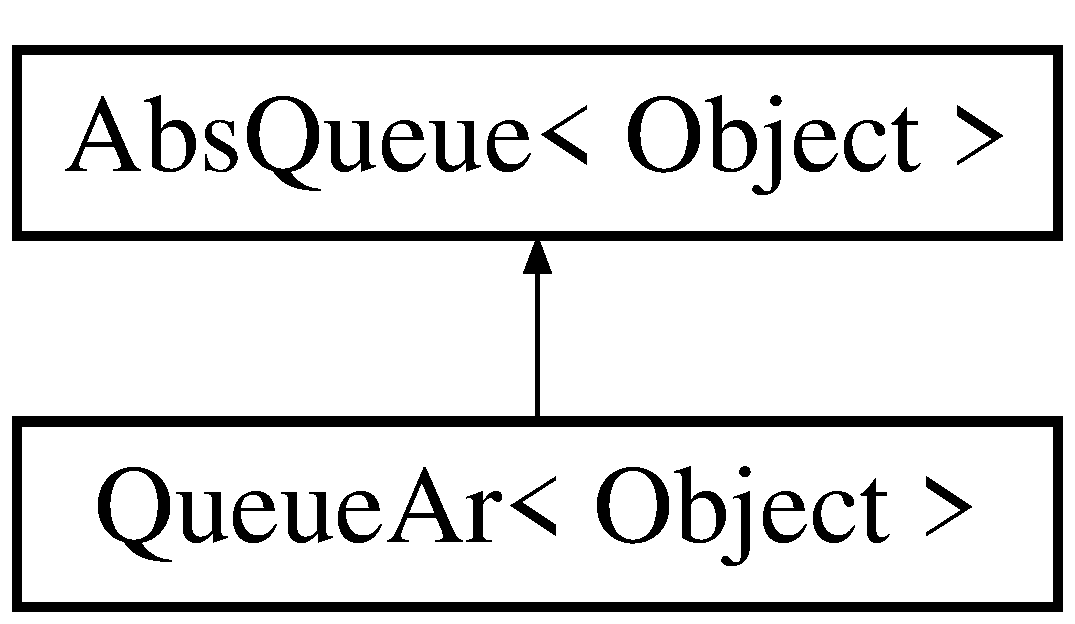
\includegraphics[height=2.000000cm]{class_abs_queue}
\end{center}
\end{figure}
\subsection*{Public Member Functions}
\begin{DoxyCompactItemize}
\item 
virtual void {\bfseries enqueue} (const Object \&x)=0\hypertarget{class_abs_queue_a172b69c1061e87a8f723b5f35d5234fe}{}\label{class_abs_queue_a172b69c1061e87a8f723b5f35d5234fe}

\item 
virtual Object {\bfseries dequeue} ()=0\hypertarget{class_abs_queue_a99c6bc5d463ea6c4c2b9cffa8c0a703b}{}\label{class_abs_queue_a99c6bc5d463ea6c4c2b9cffa8c0a703b}

\item 
virtual Object {\bfseries get\+Front} () const  =0\hypertarget{class_abs_queue_aa86da1126800e6bf2d363240ed858f4c}{}\label{class_abs_queue_aa86da1126800e6bf2d363240ed858f4c}

\item 
virtual bool {\bfseries is\+Empty} () const  =0\hypertarget{class_abs_queue_a012d3e8ad9ff8866a7ad2d75729ae3ba}{}\label{class_abs_queue_a012d3e8ad9ff8866a7ad2d75729ae3ba}

\item 
virtual void {\bfseries make\+Empty} ()=0\hypertarget{class_abs_queue_ac62860b01e9dc68fa6f4e6f217eb5e4f}{}\label{class_abs_queue_ac62860b01e9dc68fa6f4e6f217eb5e4f}

\item 
{\bfseries Abs\+Queue} (const \hyperlink{class_abs_queue}{Abs\+Queue} \&)\hypertarget{class_abs_queue_afe212750016489b7c2de53e61e30cffd}{}\label{class_abs_queue_afe212750016489b7c2de53e61e30cffd}

\end{DoxyCompactItemize}


\subsection{Detailed Description}
\subsubsection*{template$<$class Object$>$\\*
class Abs\+Queue$<$ Object $>$}

\begin{DoxyAuthor}{Author}
Selan R. 
\end{DoxyAuthor}


The documentation for this class was generated from the following file\+:\begin{DoxyCompactItemize}
\item 
include/Abs\+Queue.\+h\end{DoxyCompactItemize}

\hypertarget{class_abs_stack}{}\section{Abs\+Stack$<$ Object $>$ Class Template Reference}
\label{class_abs_stack}\index{Abs\+Stack$<$ Object $>$@{Abs\+Stack$<$ Object $>$}}


{\ttfamily \#include $<$Abs\+Stack.\+h$>$}

Inheritance diagram for Abs\+Stack$<$ Object $>$\+:\begin{figure}[H]
\begin{center}
\leavevmode
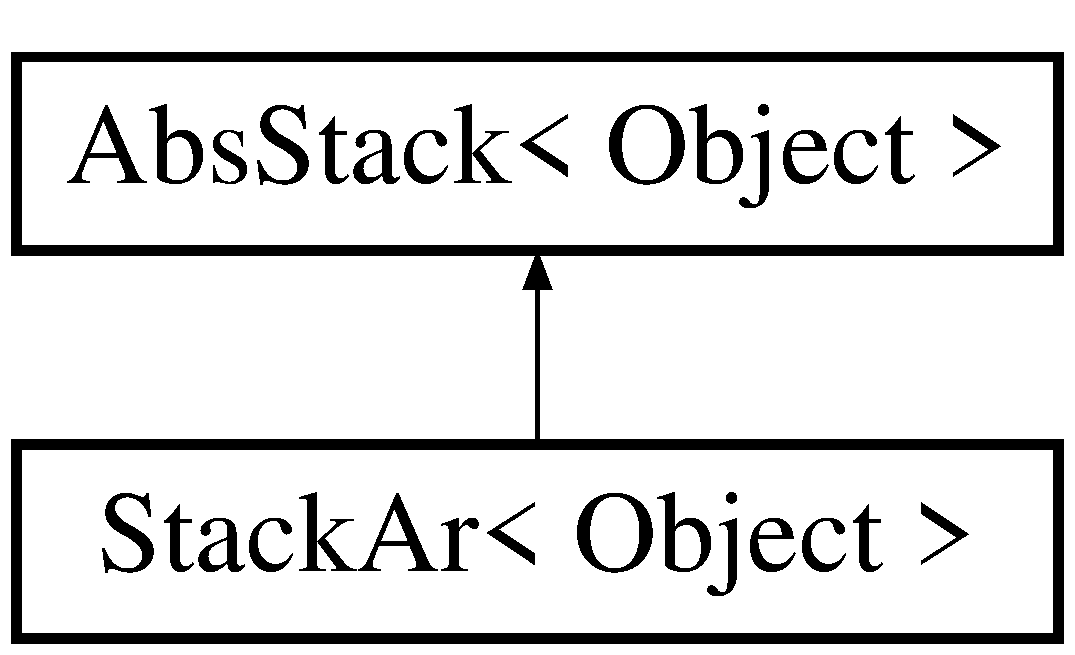
\includegraphics[height=2.000000cm]{class_abs_stack}
\end{center}
\end{figure}
\subsection*{Public Member Functions}
\begin{DoxyCompactItemize}
\item 
virtual void {\bfseries push} (const Object \&x)=0\hypertarget{class_abs_stack_ace9c9f220a85a96e3202af54356a8e26}{}\label{class_abs_stack_ace9c9f220a85a96e3202af54356a8e26}

\item 
virtual Object {\bfseries pop} ()=0\hypertarget{class_abs_stack_a4d93c845ee748069f7e88841ad80b864}{}\label{class_abs_stack_a4d93c845ee748069f7e88841ad80b864}

\item 
virtual Object {\bfseries top} () const  =0\hypertarget{class_abs_stack_a41a96b855f3995dacfeb58ff02b8011b}{}\label{class_abs_stack_a41a96b855f3995dacfeb58ff02b8011b}

\item 
virtual bool {\bfseries is\+Empty} () const  =0\hypertarget{class_abs_stack_a7da72befef800cb78f1d96e6e3e2886c}{}\label{class_abs_stack_a7da72befef800cb78f1d96e6e3e2886c}

\item 
virtual void {\bfseries make\+Empty} ()=0\hypertarget{class_abs_stack_a29ab79afef511d86b1d504b37b660599}{}\label{class_abs_stack_a29ab79afef511d86b1d504b37b660599}

\end{DoxyCompactItemize}


\subsection{Detailed Description}
\subsubsection*{template$<$class Object$>$\\*
class Abs\+Stack$<$ Object $>$}

\begin{DoxyAuthor}{Author}
Selan R. 
\end{DoxyAuthor}


The documentation for this class was generated from the following file\+:\begin{DoxyCompactItemize}
\item 
include/Abs\+Stack.\+h\end{DoxyCompactItemize}

\hypertarget{classconjuntura}{}\section{conjuntura Class Reference}
\label{classconjuntura}\index{conjuntura@{conjuntura}}


Classe conjuntura.  




{\ttfamily \#include $<$header.\+h$>$}

\subsection*{Public Member Functions}
\begin{DoxyCompactItemize}
\item 
\hyperlink{classconjuntura_af63277766a70ebce6534ec77c2f32eb9}{conjuntura} ()\hypertarget{classconjuntura_af63277766a70ebce6534ec77c2f32eb9}{}\label{classconjuntura_af63277766a70ebce6534ec77c2f32eb9}

\begin{DoxyCompactList}\small\item\em Construtor da classe conjuntura Cria as conjuturas. \end{DoxyCompactList}\item 
\hyperlink{classconjuntura_adc088f0e6f70c07c041533ac0b24c692}{$\sim$conjuntura} ()\hypertarget{classconjuntura_adc088f0e6f70c07c041533ac0b24c692}{}\label{classconjuntura_adc088f0e6f70c07c041533ac0b24c692}

\begin{DoxyCompactList}\small\item\em Destrutor da classe conjuntura Destroi as conjuturas. \end{DoxyCompactList}\item 
int \hyperlink{classconjuntura_acdea319e644d7e5c12d7b9c5fe891a28}{get\+\_\+precedencia} (std\+::string op) const 
\begin{DoxyCompactList}\small\item\em Colhe a precedencia dos operadores. \end{DoxyCompactList}\item 
bool \hyperlink{classconjuntura_ad431182bd209959cbc242855e17c24a6}{eh\+\_\+operador} (std\+::string op) const 
\begin{DoxyCompactList}\small\item\em Verifica se é o valor é um operador. \end{DoxyCompactList}\item 
bool \hyperlink{classconjuntura_a203d067e8788a4be7b879c2bf619e400}{eh\+\_\+operador\+\_\+antes} (char op) const 
\begin{DoxyCompactList}\small\item\em Verifica se é o valor é um operador antes da sequencia seguinte. \end{DoxyCompactList}\item 
bool \hyperlink{classconjuntura_ae6596c44980af69b76028e9e07bdbc27}{eh\+\_\+operador\+\_\+completa} (char op) const 
\begin{DoxyCompactList}\small\item\em Verifica se é o valor é um operador completamente. \end{DoxyCompactList}\item 
bool \hyperlink{classconjuntura_aa965f1bcbff1d132fd9b333a032c6e69}{eh\+\_\+digito} (char op) const 
\begin{DoxyCompactList}\small\item\em Verifica se é o valor é um dígito. \end{DoxyCompactList}\item 
int \hyperlink{classconjuntura_a8cf783aa2603fd8b5b28a813e320fb81}{aval\+Pos\+Fixa} ()
\begin{DoxyCompactList}\small\item\em Avalia a expressão afim de realizar os cálculos e obter o resultado. \end{DoxyCompactList}\item 
void \hyperlink{classconjuntura_a5ed989aef05d806b69852592832e2b64}{Infx2\+Posfx} ()
\begin{DoxyCompactList}\small\item\em Converte a expressão infixa para expressão pósfixa. \end{DoxyCompactList}\item 
bool \hyperlink{classconjuntura_a264666a5fb0a1810eeaa6d1ea59283a5}{token} (const char $\ast$aux, int t)
\begin{DoxyCompactList}\small\item\em Tokeniza o arquivo. \end{DoxyCompactList}\end{DoxyCompactItemize}


\subsection{Detailed Description}
Classe conjuntura. 

Assinaturas das funções e definição da classe conjuntura 

\subsection{Member Function Documentation}
\index{conjuntura@{conjuntura}!aval\+Pos\+Fixa@{aval\+Pos\+Fixa}}
\index{aval\+Pos\+Fixa@{aval\+Pos\+Fixa}!conjuntura@{conjuntura}}
\subsubsection[{\texorpdfstring{aval\+Pos\+Fixa()}{avalPosFixa()}}]{\setlength{\rightskip}{0pt plus 5cm}int conjuntura\+::aval\+Pos\+Fixa (
\begin{DoxyParamCaption}
{}
\end{DoxyParamCaption}
)}\hypertarget{classconjuntura_a8cf783aa2603fd8b5b28a813e320fb81}{}\label{classconjuntura_a8cf783aa2603fd8b5b28a813e320fb81}


Avalia a expressão afim de realizar os cálculos e obter o resultado. 

\begin{DoxyReturn}{Returns}
inteiro 
\end{DoxyReturn}
\index{conjuntura@{conjuntura}!eh\+\_\+digito@{eh\+\_\+digito}}
\index{eh\+\_\+digito@{eh\+\_\+digito}!conjuntura@{conjuntura}}
\subsubsection[{\texorpdfstring{eh\+\_\+digito(char op) const }{eh_digito(char op) const }}]{\setlength{\rightskip}{0pt plus 5cm}bool conjuntura\+::eh\+\_\+digito (
\begin{DoxyParamCaption}
\item[{char}]{op}
\end{DoxyParamCaption}
) const}\hypertarget{classconjuntura_aa965f1bcbff1d132fd9b333a032c6e69}{}\label{classconjuntura_aa965f1bcbff1d132fd9b333a032c6e69}


Verifica se é o valor é um dígito. 


\begin{DoxyParams}{Parameters}
{\em op} & Operador char usado para verificação \\
\hline
\end{DoxyParams}
\begin{DoxyReturn}{Returns}
true ou false 
\end{DoxyReturn}
\index{conjuntura@{conjuntura}!eh\+\_\+operador@{eh\+\_\+operador}}
\index{eh\+\_\+operador@{eh\+\_\+operador}!conjuntura@{conjuntura}}
\subsubsection[{\texorpdfstring{eh\+\_\+operador(std\+::string op) const }{eh_operador(std::string op) const }}]{\setlength{\rightskip}{0pt plus 5cm}bool conjuntura\+::eh\+\_\+operador (
\begin{DoxyParamCaption}
\item[{std\+::string}]{op}
\end{DoxyParamCaption}
) const}\hypertarget{classconjuntura_ad431182bd209959cbc242855e17c24a6}{}\label{classconjuntura_ad431182bd209959cbc242855e17c24a6}


Verifica se é o valor é um operador. 


\begin{DoxyParams}{Parameters}
{\em op} & Operador string usado para verificação \\
\hline
\end{DoxyParams}
\begin{DoxyReturn}{Returns}
true ou false 
\end{DoxyReturn}
\index{conjuntura@{conjuntura}!eh\+\_\+operador\+\_\+antes@{eh\+\_\+operador\+\_\+antes}}
\index{eh\+\_\+operador\+\_\+antes@{eh\+\_\+operador\+\_\+antes}!conjuntura@{conjuntura}}
\subsubsection[{\texorpdfstring{eh\+\_\+operador\+\_\+antes(char op) const }{eh_operador_antes(char op) const }}]{\setlength{\rightskip}{0pt plus 5cm}bool conjuntura\+::eh\+\_\+operador\+\_\+antes (
\begin{DoxyParamCaption}
\item[{char}]{op}
\end{DoxyParamCaption}
) const}\hypertarget{classconjuntura_a203d067e8788a4be7b879c2bf619e400}{}\label{classconjuntura_a203d067e8788a4be7b879c2bf619e400}


Verifica se é o valor é um operador antes da sequencia seguinte. 


\begin{DoxyParams}{Parameters}
{\em op} & Operador char usado para verificação \\
\hline
\end{DoxyParams}
\begin{DoxyReturn}{Returns}
true ou false 
\end{DoxyReturn}
\index{conjuntura@{conjuntura}!eh\+\_\+operador\+\_\+completa@{eh\+\_\+operador\+\_\+completa}}
\index{eh\+\_\+operador\+\_\+completa@{eh\+\_\+operador\+\_\+completa}!conjuntura@{conjuntura}}
\subsubsection[{\texorpdfstring{eh\+\_\+operador\+\_\+completa(char op) const }{eh_operador_completa(char op) const }}]{\setlength{\rightskip}{0pt plus 5cm}bool conjuntura\+::eh\+\_\+operador\+\_\+completa (
\begin{DoxyParamCaption}
\item[{char}]{op}
\end{DoxyParamCaption}
) const}\hypertarget{classconjuntura_ae6596c44980af69b76028e9e07bdbc27}{}\label{classconjuntura_ae6596c44980af69b76028e9e07bdbc27}


Verifica se é o valor é um operador completamente. 


\begin{DoxyParams}{Parameters}
{\em op} & Operador char usado para verificação \\
\hline
\end{DoxyParams}
\begin{DoxyReturn}{Returns}
true ou false 
\end{DoxyReturn}
\index{conjuntura@{conjuntura}!get\+\_\+precedencia@{get\+\_\+precedencia}}
\index{get\+\_\+precedencia@{get\+\_\+precedencia}!conjuntura@{conjuntura}}
\subsubsection[{\texorpdfstring{get\+\_\+precedencia(std\+::string op) const }{get_precedencia(std::string op) const }}]{\setlength{\rightskip}{0pt plus 5cm}int conjuntura\+::get\+\_\+precedencia (
\begin{DoxyParamCaption}
\item[{std\+::string}]{op}
\end{DoxyParamCaption}
) const}\hypertarget{classconjuntura_acdea319e644d7e5c12d7b9c5fe891a28}{}\label{classconjuntura_acdea319e644d7e5c12d7b9c5fe891a28}


Colhe a precedencia dos operadores. 


\begin{DoxyParams}{Parameters}
{\em op} & Operador string usado para verificação de precedência \\
\hline
\end{DoxyParams}
\begin{DoxyReturn}{Returns}
Um inteiro equivalente a sua precedencia Precedencia Operadores 1 -\/(un) 2 ˆ 3 $\ast$ / \% 4 + -\/ 5 () 
\end{DoxyReturn}
\index{conjuntura@{conjuntura}!Infx2\+Posfx@{Infx2\+Posfx}}
\index{Infx2\+Posfx@{Infx2\+Posfx}!conjuntura@{conjuntura}}
\subsubsection[{\texorpdfstring{Infx2\+Posfx()}{Infx2Posfx()}}]{\setlength{\rightskip}{0pt plus 5cm}void conjuntura\+::\+Infx2\+Posfx (
\begin{DoxyParamCaption}
{}
\end{DoxyParamCaption}
)}\hypertarget{classconjuntura_a5ed989aef05d806b69852592832e2b64}{}\label{classconjuntura_a5ed989aef05d806b69852592832e2b64}


Converte a expressão infixa para expressão pósfixa. 

\begin{DoxyReturn}{Returns}
void 
\end{DoxyReturn}
\index{conjuntura@{conjuntura}!token@{token}}
\index{token@{token}!conjuntura@{conjuntura}}
\subsubsection[{\texorpdfstring{token(const char $\ast$aux, int t)}{token(const char *aux, int t)}}]{\setlength{\rightskip}{0pt plus 5cm}bool conjuntura\+::token (
\begin{DoxyParamCaption}
\item[{const char $\ast$}]{aux, }
\item[{int}]{t}
\end{DoxyParamCaption}
)}\hypertarget{classconjuntura_a264666a5fb0a1810eeaa6d1ea59283a5}{}\label{classconjuntura_a264666a5fb0a1810eeaa6d1ea59283a5}


Tokeniza o arquivo. 


\begin{DoxyParams}{Parameters}
{\em aux} & Recebe um vetor char do arquivo via getline. \\
\hline
{\em t} & Tamanho da string. \\
\hline
\end{DoxyParams}
\begin{DoxyReturn}{Returns}
True caso a expressão seja correta e False caso contrário 
\end{DoxyReturn}


The documentation for this class was generated from the following files\+:\begin{DoxyCompactItemize}
\item 
include/\hyperlink{header_8h}{header.\+h}\item 
include/\hyperlink{header_8inl}{header.\+inl}\end{DoxyCompactItemize}

\hypertarget{class_queue_ar}{}\section{Queue\+Ar$<$ Object $>$ Class Template Reference}
\label{class_queue_ar}\index{Queue\+Ar$<$ Object $>$@{Queue\+Ar$<$ Object $>$}}


Classe \hyperlink{class_queue_ar}{Queue\+Ar}.  




{\ttfamily \#include $<$queuear.\+h$>$}

Inheritance diagram for Queue\+Ar$<$ Object $>$\+:\begin{figure}[H]
\begin{center}
\leavevmode
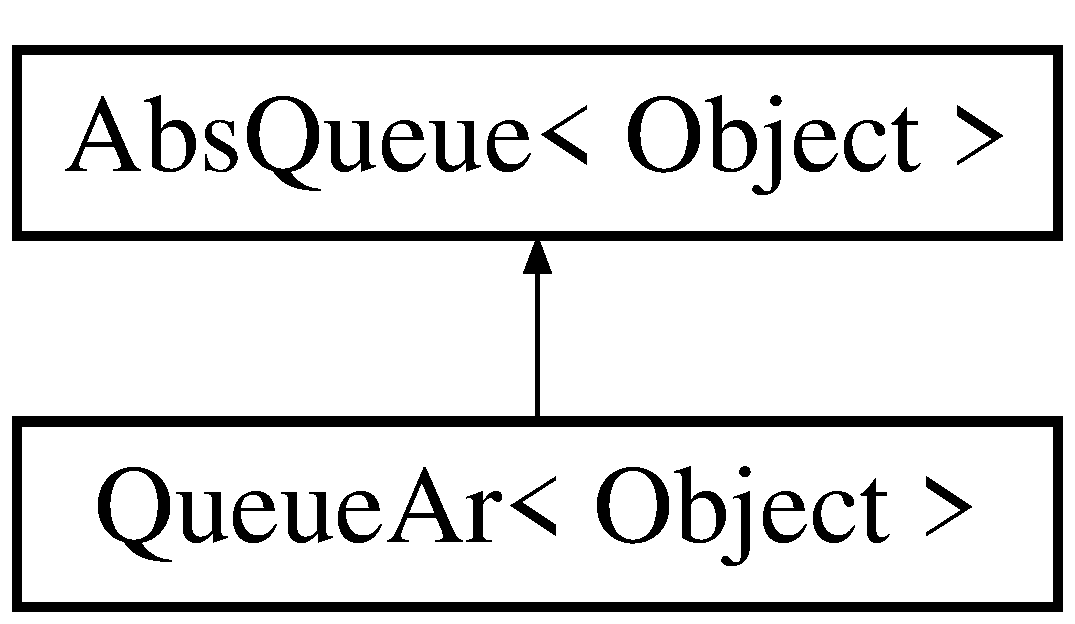
\includegraphics[height=2.000000cm]{class_queue_ar}
\end{center}
\end{figure}
\subsection*{Public Member Functions}
\begin{DoxyCompactItemize}
\item 
\hyperlink{class_queue_ar_aff2b7644e32ec281d312939aa775faec}{Queue\+Ar} (const int \+\_\+size=10)
\begin{DoxyCompactList}\small\item\em Construtor \hyperlink{class_queue_ar}{Queue\+Ar}. \end{DoxyCompactList}\item 
\hyperlink{class_queue_ar_a4f5e5ac9bcc103787ddf13247c401819}{$\sim$\+Queue\+Ar} ()\hypertarget{class_queue_ar_a4f5e5ac9bcc103787ddf13247c401819}{}\label{class_queue_ar_a4f5e5ac9bcc103787ddf13247c401819}

\begin{DoxyCompactList}\small\item\em Destrutor da classe \hyperlink{class_queue_ar}{Queue\+Ar} Destroi a fila. \end{DoxyCompactList}\item 
void \hyperlink{class_queue_ar_a4d5801295edee5f26a730ae8e2bc0675}{enqueue} (const Object \&x)
\begin{DoxyCompactList}\small\item\em Insere elementos na fila. \end{DoxyCompactList}\item 
Object \hyperlink{class_queue_ar_aa8bef4597ae7b4efbaec8f6866eb8342}{dequeue} ()
\begin{DoxyCompactList}\small\item\em Remove elementos da fila. \end{DoxyCompactList}\item 
Object \hyperlink{class_queue_ar_ad79382827047677e605fe2c905792edb}{get\+Front} () const 
\begin{DoxyCompactList}\small\item\em Pega o elemento que está na guarda da fila. \end{DoxyCompactList}\item 
Object \hyperlink{class_queue_ar_a5c9bd4407de280c789c18a25ccb61a5b}{get\+Back} () const 
\begin{DoxyCompactList}\small\item\em Pega o elemento que está na retaguarda da fila. \end{DoxyCompactList}\item 
bool \hyperlink{class_queue_ar_adc5f98078020d631ac866fffc19d6d28}{is\+Empty} () const 
\begin{DoxyCompactList}\small\item\em Verifica se a fila está vazia \{ \}. \end{DoxyCompactList}\item 
void \hyperlink{class_queue_ar_ae95415c3620c41922ec87a778d6b55fb}{make\+Empty} ()
\begin{DoxyCompactList}\small\item\em Limpa toda a fila. \end{DoxyCompactList}\end{DoxyCompactItemize}
\subsection*{Friends}
\begin{DoxyCompactItemize}
\item 
std\+::ostream \& \hyperlink{class_queue_ar_a75d13432fdce3268265b40ceafa779cb}{operator$<$$<$} (std\+::ostream \&op, const \hyperlink{class_queue_ar}{Queue\+Ar} \&obj)
\begin{DoxyCompactList}\small\item\em Sobrecarga do operador $<$$<$ para a fila. \end{DoxyCompactList}\end{DoxyCompactItemize}


\subsection{Detailed Description}
\subsubsection*{template$<$class Object$>$\\*
class Queue\+Ar$<$ Object $>$}

Classe \hyperlink{class_queue_ar}{Queue\+Ar}. 

Implementação e assinatura das funções da classe \hyperlink{class_queue_ar}{Queue\+Ar} 

\subsection{Constructor \& Destructor Documentation}
\index{Queue\+Ar@{Queue\+Ar}!Queue\+Ar@{Queue\+Ar}}
\index{Queue\+Ar@{Queue\+Ar}!Queue\+Ar@{Queue\+Ar}}
\subsubsection[{\texorpdfstring{Queue\+Ar(const int \+\_\+size=10)}{QueueAr(const int _size=10)}}]{\setlength{\rightskip}{0pt plus 5cm}template$<$class Object $>$ {\bf Queue\+Ar}$<$ Object $>$\+::{\bf Queue\+Ar} (
\begin{DoxyParamCaption}
\item[{const int}]{\+\_\+size = {\ttfamily 10}}
\end{DoxyParamCaption}
)}\hypertarget{class_queue_ar_aff2b7644e32ec281d312939aa775faec}{}\label{class_queue_ar_aff2b7644e32ec281d312939aa775faec}


Construtor \hyperlink{class_queue_ar}{Queue\+Ar}. 


\begin{DoxyParams}{Parameters}
{\em \+\_\+size} & \\
\hline
\end{DoxyParams}
Seta as Variáveis da classe e tem tamanho padrão 10 

\subsection{Member Function Documentation}
\index{Queue\+Ar@{Queue\+Ar}!dequeue@{dequeue}}
\index{dequeue@{dequeue}!Queue\+Ar@{Queue\+Ar}}
\subsubsection[{\texorpdfstring{dequeue()}{dequeue()}}]{\setlength{\rightskip}{0pt plus 5cm}template$<$class Object $>$ Object {\bf Queue\+Ar}$<$ Object $>$\+::dequeue (
\begin{DoxyParamCaption}
{}
\end{DoxyParamCaption}
)\hspace{0.3cm}{\ttfamily [virtual]}}\hypertarget{class_queue_ar_aa8bef4597ae7b4efbaec8f6866eb8342}{}\label{class_queue_ar_aa8bef4597ae7b4efbaec8f6866eb8342}


Remove elementos da fila. 


\begin{DoxyParams}{Parameters}
{\em x} & Elemento a ser removido \\
\hline
\end{DoxyParams}
\begin{DoxyReturn}{Returns}
void 
\end{DoxyReturn}


Implements \hyperlink{class_abs_queue}{Abs\+Queue$<$ Object $>$}.

\index{Queue\+Ar@{Queue\+Ar}!enqueue@{enqueue}}
\index{enqueue@{enqueue}!Queue\+Ar@{Queue\+Ar}}
\subsubsection[{\texorpdfstring{enqueue(const Object \&x)}{enqueue(const Object &x)}}]{\setlength{\rightskip}{0pt plus 5cm}template$<$class Object$>$ void {\bf Queue\+Ar}$<$ Object $>$\+::enqueue (
\begin{DoxyParamCaption}
\item[{const Object \&}]{x}
\end{DoxyParamCaption}
)\hspace{0.3cm}{\ttfamily [virtual]}}\hypertarget{class_queue_ar_a4d5801295edee5f26a730ae8e2bc0675}{}\label{class_queue_ar_a4d5801295edee5f26a730ae8e2bc0675}


Insere elementos na fila. 


\begin{DoxyParams}{Parameters}
{\em x} & Recebe o elemento a ser adicionado \\
\hline
\end{DoxyParams}
\begin{DoxyReturn}{Returns}
void 
\end{DoxyReturn}


Implements \hyperlink{class_abs_queue}{Abs\+Queue$<$ Object $>$}.

\index{Queue\+Ar@{Queue\+Ar}!get\+Back@{get\+Back}}
\index{get\+Back@{get\+Back}!Queue\+Ar@{Queue\+Ar}}
\subsubsection[{\texorpdfstring{get\+Back() const }{getBack() const }}]{\setlength{\rightskip}{0pt plus 5cm}template$<$class Object $>$ Object {\bf Queue\+Ar}$<$ Object $>$\+::get\+Back (
\begin{DoxyParamCaption}
{}
\end{DoxyParamCaption}
) const}\hypertarget{class_queue_ar_a5c9bd4407de280c789c18a25ccb61a5b}{}\label{class_queue_ar_a5c9bd4407de280c789c18a25ccb61a5b}


Pega o elemento que está na retaguarda da fila. 

\begin{DoxyReturn}{Returns}
Elemento de trás 
\end{DoxyReturn}
\index{Queue\+Ar@{Queue\+Ar}!get\+Front@{get\+Front}}
\index{get\+Front@{get\+Front}!Queue\+Ar@{Queue\+Ar}}
\subsubsection[{\texorpdfstring{get\+Front() const }{getFront() const }}]{\setlength{\rightskip}{0pt plus 5cm}template$<$class Object $>$ Object {\bf Queue\+Ar}$<$ Object $>$\+::get\+Front (
\begin{DoxyParamCaption}
{}
\end{DoxyParamCaption}
) const\hspace{0.3cm}{\ttfamily [virtual]}}\hypertarget{class_queue_ar_ad79382827047677e605fe2c905792edb}{}\label{class_queue_ar_ad79382827047677e605fe2c905792edb}


Pega o elemento que está na guarda da fila. 

\begin{DoxyReturn}{Returns}
Elemento da frente 
\end{DoxyReturn}


Implements \hyperlink{class_abs_queue}{Abs\+Queue$<$ Object $>$}.

\index{Queue\+Ar@{Queue\+Ar}!is\+Empty@{is\+Empty}}
\index{is\+Empty@{is\+Empty}!Queue\+Ar@{Queue\+Ar}}
\subsubsection[{\texorpdfstring{is\+Empty() const }{isEmpty() const }}]{\setlength{\rightskip}{0pt plus 5cm}template$<$class Object $>$ bool {\bf Queue\+Ar}$<$ Object $>$\+::is\+Empty (
\begin{DoxyParamCaption}
{}
\end{DoxyParamCaption}
) const\hspace{0.3cm}{\ttfamily [virtual]}}\hypertarget{class_queue_ar_adc5f98078020d631ac866fffc19d6d28}{}\label{class_queue_ar_adc5f98078020d631ac866fffc19d6d28}


Verifica se a fila está vazia \{ \}. 

\begin{DoxyReturn}{Returns}
True se a fila estiver vazia ou False se a fila não estiver vazia 
\end{DoxyReturn}


Implements \hyperlink{class_abs_queue}{Abs\+Queue$<$ Object $>$}.

\index{Queue\+Ar@{Queue\+Ar}!make\+Empty@{make\+Empty}}
\index{make\+Empty@{make\+Empty}!Queue\+Ar@{Queue\+Ar}}
\subsubsection[{\texorpdfstring{make\+Empty()}{makeEmpty()}}]{\setlength{\rightskip}{0pt plus 5cm}template$<$class Object $>$ void {\bf Queue\+Ar}$<$ Object $>$\+::make\+Empty (
\begin{DoxyParamCaption}
{}
\end{DoxyParamCaption}
)\hspace{0.3cm}{\ttfamily [virtual]}}\hypertarget{class_queue_ar_ae95415c3620c41922ec87a778d6b55fb}{}\label{class_queue_ar_ae95415c3620c41922ec87a778d6b55fb}


Limpa toda a fila. 

\begin{DoxyReturn}{Returns}
void 
\end{DoxyReturn}


Implements \hyperlink{class_abs_queue}{Abs\+Queue$<$ Object $>$}.



\subsection{Friends And Related Function Documentation}
\index{Queue\+Ar@{Queue\+Ar}!operator$<$$<$@{operator$<$$<$}}
\index{operator$<$$<$@{operator$<$$<$}!Queue\+Ar@{Queue\+Ar}}
\subsubsection[{\texorpdfstring{operator$<$$<$}{operator<<}}]{\setlength{\rightskip}{0pt plus 5cm}template$<$class Object$>$ std\+::ostream\& operator$<$$<$ (
\begin{DoxyParamCaption}
\item[{std\+::ostream \&}]{op, }
\item[{const {\bf Queue\+Ar}$<$ Object $>$ \&}]{obj}
\end{DoxyParamCaption}
)\hspace{0.3cm}{\ttfamily [friend]}}\hypertarget{class_queue_ar_a75d13432fdce3268265b40ceafa779cb}{}\label{class_queue_ar_a75d13432fdce3268265b40ceafa779cb}


Sobrecarga do operador $<$$<$ para a fila. 


\begin{DoxyParams}{Parameters}
{\em op} & std\+::ostream \\
\hline
{\em obj} & Objeto da classe \hyperlink{class_queue_ar}{Queue\+Ar} \\
\hline
\end{DoxyParams}
\begin{DoxyReturn}{Returns}
std\+::ostream op 
\end{DoxyReturn}


The documentation for this class was generated from the following files\+:\begin{DoxyCompactItemize}
\item 
include/\hyperlink{queuear_8h}{queuear.\+h}\item 
include/\hyperlink{queuear_8inl}{queuear.\+inl}\end{DoxyCompactItemize}

\hypertarget{class_stack_ar}{}\section{Stack\+Ar$<$ Object $>$ Class Template Reference}
\label{class_stack_ar}\index{Stack\+Ar$<$ Object $>$@{Stack\+Ar$<$ Object $>$}}


Classe \hyperlink{class_stack_ar}{Stack\+Ar}.  




{\ttfamily \#include $<$stackar.\+h$>$}

Inheritance diagram for Stack\+Ar$<$ Object $>$\+:\begin{figure}[H]
\begin{center}
\leavevmode
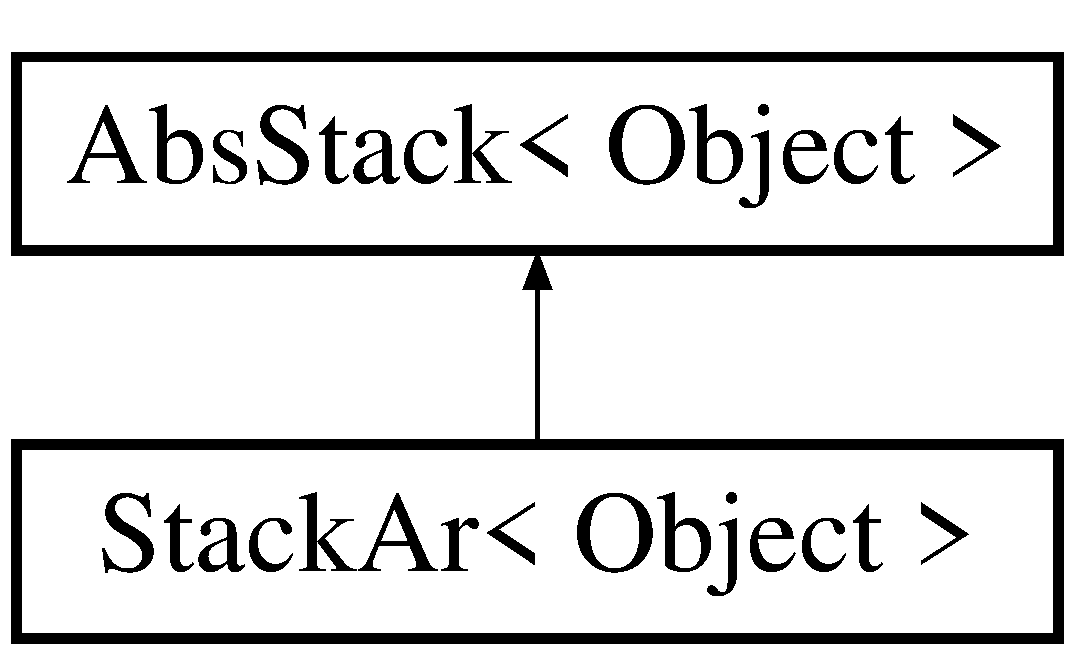
\includegraphics[height=2.000000cm]{class_stack_ar}
\end{center}
\end{figure}
\subsection*{Public Member Functions}
\begin{DoxyCompactItemize}
\item 
\hyperlink{class_stack_ar_ae1256302064835dbd36d078902670b5e}{Stack\+Ar} (const int \&\+\_\+size=10)
\begin{DoxyCompactList}\small\item\em Construtor \hyperlink{class_stack_ar}{Stack\+Ar}. \end{DoxyCompactList}\item 
\hyperlink{class_stack_ar_a4ad1d77653d6ebfbe03bb359f610863c}{$\sim$\+Stack\+Ar} ()\hypertarget{class_stack_ar_a4ad1d77653d6ebfbe03bb359f610863c}{}\label{class_stack_ar_a4ad1d77653d6ebfbe03bb359f610863c}

\begin{DoxyCompactList}\small\item\em Destrutor da classe \hyperlink{class_queue_ar}{Queue\+Ar} Destroi a Pilha. \end{DoxyCompactList}\item 
void \hyperlink{class_stack_ar_ad3fc10de870f4ef52fb37f0a9b335222}{push} (const Object \&x)
\begin{DoxyCompactList}\small\item\em Insere elementos na pilha. \end{DoxyCompactList}\item 
Object \hyperlink{class_stack_ar_a53d0e26536ad28e464b8bf99f84d8760}{pop} ()
\begin{DoxyCompactList}\small\item\em Remove o elemento no topo da pilha. \end{DoxyCompactList}\item 
Object \hyperlink{class_stack_ar_a15a4938f80dc4009aaba5eb01bd1e6c1}{top} () const 
\begin{DoxyCompactList}\small\item\em Retorna o elemento no topo da pilha. \end{DoxyCompactList}\item 
Object \hyperlink{class_stack_ar_a6f12b2c8213a6935cfb7ecf7d4875210}{get\+Capacidade} () const 
\begin{DoxyCompactList}\small\item\em Pega o tamanho da capacidade da pilha. \end{DoxyCompactList}\item 
bool \hyperlink{class_stack_ar_ae4dcecdf54a3f6ed7cf9192cec8c60a5}{is\+Empty} () const 
\begin{DoxyCompactList}\small\item\em Verifica se a pilha está vazia \{ \}. \end{DoxyCompactList}\item 
void \hyperlink{class_stack_ar_ac6252abb241ee6d9c827eabd4519fdb8}{make\+Empty} ()
\begin{DoxyCompactList}\small\item\em Apaga toda a pilha. \end{DoxyCompactList}\item 
void {\bfseries print} ()\hypertarget{class_stack_ar_a1e3e5bd273aa6034dd0f95d6a00f6220}{}\label{class_stack_ar_a1e3e5bd273aa6034dd0f95d6a00f6220}

\end{DoxyCompactItemize}
\subsection*{Friends}
\begin{DoxyCompactItemize}
\item 
std\+::ostream \& \hyperlink{class_stack_ar_ace3850b785f09b70ff174a57cadd4a96}{operator$<$$<$} (std\+::ostream \&op, const \hyperlink{class_stack_ar}{Stack\+Ar} \&objeto)
\begin{DoxyCompactList}\small\item\em Sobrecarga do operador $<$$<$ para a pilha. \end{DoxyCompactList}\end{DoxyCompactItemize}


\subsection{Detailed Description}
\subsubsection*{template$<$class Object$>$\\*
class Stack\+Ar$<$ Object $>$}

Classe \hyperlink{class_stack_ar}{Stack\+Ar}. 

Implementação e assinatura das funções da classe \hyperlink{class_queue_ar}{Queue\+Ar} 

\subsection{Constructor \& Destructor Documentation}
\index{Stack\+Ar@{Stack\+Ar}!Stack\+Ar@{Stack\+Ar}}
\index{Stack\+Ar@{Stack\+Ar}!Stack\+Ar@{Stack\+Ar}}
\subsubsection[{\texorpdfstring{Stack\+Ar(const int \&\+\_\+size=10)}{StackAr(const int &_size=10)}}]{\setlength{\rightskip}{0pt plus 5cm}template$<$class Object $>$ {\bf Stack\+Ar}$<$ Object $>$\+::{\bf Stack\+Ar} (
\begin{DoxyParamCaption}
\item[{const int \&}]{\+\_\+size = {\ttfamily 10}}
\end{DoxyParamCaption}
)}\hypertarget{class_stack_ar_ae1256302064835dbd36d078902670b5e}{}\label{class_stack_ar_ae1256302064835dbd36d078902670b5e}


Construtor \hyperlink{class_stack_ar}{Stack\+Ar}. 


\begin{DoxyParams}{Parameters}
{\em \+\_\+size} & \\
\hline
\end{DoxyParams}
Seta as Variáveis da classe e tem tamanho padrão 10 

\subsection{Member Function Documentation}
\index{Stack\+Ar@{Stack\+Ar}!get\+Capacidade@{get\+Capacidade}}
\index{get\+Capacidade@{get\+Capacidade}!Stack\+Ar@{Stack\+Ar}}
\subsubsection[{\texorpdfstring{get\+Capacidade() const }{getCapacidade() const }}]{\setlength{\rightskip}{0pt plus 5cm}template$<$class Object $>$ Object {\bf Stack\+Ar}$<$ Object $>$\+::get\+Capacidade (
\begin{DoxyParamCaption}
{}
\end{DoxyParamCaption}
) const}\hypertarget{class_stack_ar_a6f12b2c8213a6935cfb7ecf7d4875210}{}\label{class_stack_ar_a6f12b2c8213a6935cfb7ecf7d4875210}


Pega o tamanho da capacidade da pilha. 

\begin{DoxyReturn}{Returns}
O tamanho da capacidade da pilha 
\end{DoxyReturn}
\index{Stack\+Ar@{Stack\+Ar}!is\+Empty@{is\+Empty}}
\index{is\+Empty@{is\+Empty}!Stack\+Ar@{Stack\+Ar}}
\subsubsection[{\texorpdfstring{is\+Empty() const }{isEmpty() const }}]{\setlength{\rightskip}{0pt plus 5cm}template$<$class Object $>$ bool {\bf Stack\+Ar}$<$ Object $>$\+::is\+Empty (
\begin{DoxyParamCaption}
{}
\end{DoxyParamCaption}
) const\hspace{0.3cm}{\ttfamily [inline]}, {\ttfamily [virtual]}}\hypertarget{class_stack_ar_ae4dcecdf54a3f6ed7cf9192cec8c60a5}{}\label{class_stack_ar_ae4dcecdf54a3f6ed7cf9192cec8c60a5}


Verifica se a pilha está vazia \{ \}. 

\begin{DoxyReturn}{Returns}
True se a pilha estiver vazia e False caso haja elementos 
\end{DoxyReturn}


Implements \hyperlink{class_abs_stack}{Abs\+Stack$<$ Object $>$}.

\index{Stack\+Ar@{Stack\+Ar}!make\+Empty@{make\+Empty}}
\index{make\+Empty@{make\+Empty}!Stack\+Ar@{Stack\+Ar}}
\subsubsection[{\texorpdfstring{make\+Empty()}{makeEmpty()}}]{\setlength{\rightskip}{0pt plus 5cm}template$<$class Object $>$ void {\bf Stack\+Ar}$<$ Object $>$\+::make\+Empty (
\begin{DoxyParamCaption}
{}
\end{DoxyParamCaption}
)\hspace{0.3cm}{\ttfamily [inline]}, {\ttfamily [virtual]}}\hypertarget{class_stack_ar_ac6252abb241ee6d9c827eabd4519fdb8}{}\label{class_stack_ar_ac6252abb241ee6d9c827eabd4519fdb8}


Apaga toda a pilha. 

\begin{DoxyReturn}{Returns}
void 
\end{DoxyReturn}


Implements \hyperlink{class_abs_stack}{Abs\+Stack$<$ Object $>$}.

\index{Stack\+Ar@{Stack\+Ar}!pop@{pop}}
\index{pop@{pop}!Stack\+Ar@{Stack\+Ar}}
\subsubsection[{\texorpdfstring{pop()}{pop()}}]{\setlength{\rightskip}{0pt plus 5cm}template$<$class Object $>$ Object {\bf Stack\+Ar}$<$ Object $>$\+::pop (
\begin{DoxyParamCaption}
\item[{void}]{}
\end{DoxyParamCaption}
)\hspace{0.3cm}{\ttfamily [virtual]}}\hypertarget{class_stack_ar_a53d0e26536ad28e464b8bf99f84d8760}{}\label{class_stack_ar_a53d0e26536ad28e464b8bf99f84d8760}


Remove o elemento no topo da pilha. 

\begin{DoxyReturn}{Returns}
void 
\end{DoxyReturn}


Implements \hyperlink{class_abs_stack}{Abs\+Stack$<$ Object $>$}.

\index{Stack\+Ar@{Stack\+Ar}!push@{push}}
\index{push@{push}!Stack\+Ar@{Stack\+Ar}}
\subsubsection[{\texorpdfstring{push(const Object \&x)}{push(const Object &x)}}]{\setlength{\rightskip}{0pt plus 5cm}template$<$class Object $>$ void {\bf Stack\+Ar}$<$ Object $>$\+::push (
\begin{DoxyParamCaption}
\item[{const Object \&}]{x}
\end{DoxyParamCaption}
)\hspace{0.3cm}{\ttfamily [virtual]}}\hypertarget{class_stack_ar_ad3fc10de870f4ef52fb37f0a9b335222}{}\label{class_stack_ar_ad3fc10de870f4ef52fb37f0a9b335222}


Insere elementos na pilha. 


\begin{DoxyParams}{Parameters}
{\em x} & Recebe o elemento a ser adicionado \\
\hline
\end{DoxyParams}
\begin{DoxyReturn}{Returns}
void 
\end{DoxyReturn}


Implements \hyperlink{class_abs_stack}{Abs\+Stack$<$ Object $>$}.

\index{Stack\+Ar@{Stack\+Ar}!top@{top}}
\index{top@{top}!Stack\+Ar@{Stack\+Ar}}
\subsubsection[{\texorpdfstring{top() const }{top() const }}]{\setlength{\rightskip}{0pt plus 5cm}template$<$class Object $>$ Object {\bf Stack\+Ar}$<$ Object $>$\+::top (
\begin{DoxyParamCaption}
{}
\end{DoxyParamCaption}
) const\hspace{0.3cm}{\ttfamily [virtual]}}\hypertarget{class_stack_ar_a15a4938f80dc4009aaba5eb01bd1e6c1}{}\label{class_stack_ar_a15a4938f80dc4009aaba5eb01bd1e6c1}


Retorna o elemento no topo da pilha. 

\begin{DoxyReturn}{Returns}
Elemento no topo da pilha 
\end{DoxyReturn}


Implements \hyperlink{class_abs_stack}{Abs\+Stack$<$ Object $>$}.



\subsection{Friends And Related Function Documentation}
\index{Stack\+Ar@{Stack\+Ar}!operator$<$$<$@{operator$<$$<$}}
\index{operator$<$$<$@{operator$<$$<$}!Stack\+Ar@{Stack\+Ar}}
\subsubsection[{\texorpdfstring{operator$<$$<$}{operator<<}}]{\setlength{\rightskip}{0pt plus 5cm}template$<$class Object $>$ std\+::ostream\& operator$<$$<$ (
\begin{DoxyParamCaption}
\item[{std\+::ostream \&}]{op, }
\item[{const {\bf Stack\+Ar}$<$ Object $>$ \&}]{objeto}
\end{DoxyParamCaption}
)\hspace{0.3cm}{\ttfamily [friend]}}\hypertarget{class_stack_ar_ace3850b785f09b70ff174a57cadd4a96}{}\label{class_stack_ar_ace3850b785f09b70ff174a57cadd4a96}


Sobrecarga do operador $<$$<$ para a pilha. 


\begin{DoxyParams}{Parameters}
{\em op} & std\+::ostream \\
\hline
{\em objeto} & Objeto da classe \hyperlink{class_queue_ar}{Queue\+Ar} \\
\hline
\end{DoxyParams}
\begin{DoxyReturn}{Returns}
std\+::ostream op 
\end{DoxyReturn}


The documentation for this class was generated from the following files\+:\begin{DoxyCompactItemize}
\item 
include/\hyperlink{stackar_8h}{stackar.\+h}\item 
include/\hyperlink{stackar_8inl}{stackar.\+inl}\end{DoxyCompactItemize}

\chapter{File Documentation}
\hypertarget{header_8h}{}\section{include/header.h File Reference}
\label{header_8h}\index{include/header.\+h@{include/header.\+h}}


Corpo da Classe Conjuntura.  


{\ttfamily \#include $<$iostream$>$}\\*
{\ttfamily \#include $<$string$>$}\\*
{\ttfamily \#include $<$cstring$>$}\\*
{\ttfamily \#include $<$fstream$>$}\\*
{\ttfamily \#include $<$sstream$>$}\\*
{\ttfamily \#include $<$cmath$>$}\\*
{\ttfamily \#include $<$stdlib.\+h$>$}\\*
{\ttfamily \#include \char`\"{}queuear.\+h\char`\"{}}\\*
{\ttfamily \#include \char`\"{}stackar.\+h\char`\"{}}\\*
{\ttfamily \#include \char`\"{}header.\+inl\char`\"{}}\\*
\subsection*{Classes}
\begin{DoxyCompactItemize}
\item 
class \hyperlink{classconjuntura}{conjuntura}
\begin{DoxyCompactList}\small\item\em Classe conjuntura. \end{DoxyCompactList}\end{DoxyCompactItemize}


\subsection{Detailed Description}
Corpo da Classe Conjuntura. 

Arquivo com a classe conjuntura 
\hypertarget{header_8inl}{}\section{include/header.inl File Reference}
\label{header_8inl}\index{include/header.\+inl@{include/header.\+inl}}


Implementação da Classe conjuntura.  


{\ttfamily \#include \char`\"{}header.\+h\char`\"{}}\\*


\subsection{Detailed Description}
Implementação da Classe conjuntura. 

Arquivo com a construção das funções da classe conjuntura 
\hypertarget{queuear_8h}{}\section{include/queuear.h File Reference}
\label{queuear_8h}\index{include/queuear.\+h@{include/queuear.\+h}}


Corpo da classe \hyperlink{class_queue_ar}{Queue\+Ar}.  


{\ttfamily \#include $<$iostream$>$}\\*
{\ttfamily \#include \char`\"{}Abs\+Queue.\+h\char`\"{}}\\*
{\ttfamily \#include \char`\"{}queuear.\+inl\char`\"{}}\\*
\subsection*{Classes}
\begin{DoxyCompactItemize}
\item 
class \hyperlink{class_queue_ar}{Queue\+Ar$<$ Object $>$}
\begin{DoxyCompactList}\small\item\em Classe \hyperlink{class_queue_ar}{Queue\+Ar}. \end{DoxyCompactList}\end{DoxyCompactItemize}


\subsection{Detailed Description}
Corpo da classe \hyperlink{class_queue_ar}{Queue\+Ar}. 

Arquivo com o corpo da classe \hyperlink{class_queue_ar}{Queue\+Ar} 
\hypertarget{queuear_8inl}{}\section{include/queuear.inl File Reference}
\label{queuear_8inl}\index{include/queuear.\+inl@{include/queuear.\+inl}}


Implementação da classe \hyperlink{class_queue_ar}{Queue\+Ar}.  


{\ttfamily \#include \char`\"{}queuear.\+h\char`\"{}}\\*


\subsection{Detailed Description}
Implementação da classe \hyperlink{class_queue_ar}{Queue\+Ar}. 

Arquivo com a construção das funções da classe \hyperlink{class_queue_ar}{Queue\+Ar} 
\hypertarget{stackar_8h}{}\section{include/stackar.h File Reference}
\label{stackar_8h}\index{include/stackar.\+h@{include/stackar.\+h}}


Corpo da classe \hyperlink{class_stack_ar}{Stack\+Ar}.  


{\ttfamily \#include $<$iostream$>$}\\*
{\ttfamily \#include $<$stdexcept$>$}\\*
{\ttfamily \#include \char`\"{}Abs\+Stack.\+h\char`\"{}}\\*
{\ttfamily \#include \char`\"{}stackar.\+inl\char`\"{}}\\*
\subsection*{Classes}
\begin{DoxyCompactItemize}
\item 
class \hyperlink{class_stack_ar}{Stack\+Ar$<$ Object $>$}
\begin{DoxyCompactList}\small\item\em Classe \hyperlink{class_stack_ar}{Stack\+Ar}. \end{DoxyCompactList}\end{DoxyCompactItemize}


\subsection{Detailed Description}
Corpo da classe \hyperlink{class_stack_ar}{Stack\+Ar}. 

Arquivo com o corpo da classe \hyperlink{class_stack_ar}{Stack\+Ar} 
\hypertarget{stackar_8inl}{}\section{include/stackar.inl File Reference}
\label{stackar_8inl}\index{include/stackar.\+inl@{include/stackar.\+inl}}


Implementação da classe \hyperlink{class_stack_ar}{Stack\+Ar}.  


{\ttfamily \#include $<$iostream$>$}\\*
{\ttfamily \#include $<$stdexcept$>$}\\*
{\ttfamily \#include \char`\"{}stackar.\+h\char`\"{}}\\*


\subsection{Detailed Description}
Implementação da classe \hyperlink{class_stack_ar}{Stack\+Ar}. 

Arquivo com a construção das funções da classe \hyperlink{class_stack_ar}{Stack\+Ar} 
\hypertarget{drive_8cpp}{}\section{src/drive.cpp File Reference}
\label{drive_8cpp}\index{src/drive.\+cpp@{src/drive.\+cpp}}


Arquivo Main.  


{\ttfamily \#include \char`\"{}header.\+h\char`\"{}}\\*
{\ttfamily \#include \char`\"{}queuear.\+h\char`\"{}}\\*
{\ttfamily \#include \char`\"{}stackar.\+h\char`\"{}}\\*
\subsection*{Functions}
\begin{DoxyCompactItemize}
\item 
int \hyperlink{drive_8cpp_abf9e6b7e6f15df4b525a2e7705ba3089}{main} (int argc, char const $\ast$argv\mbox{[}$\,$\mbox{]})
\begin{DoxyCompactList}\small\item\em Main. \end{DoxyCompactList}\end{DoxyCompactItemize}


\subsection{Detailed Description}
Arquivo Main. 

Arquivo com o método Main 

\subsection{Function Documentation}
\index{drive.\+cpp@{drive.\+cpp}!main@{main}}
\index{main@{main}!drive.\+cpp@{drive.\+cpp}}
\subsubsection[{\texorpdfstring{main(int argc, char const $\ast$argv[])}{main(int argc, char const *argv[])}}]{\setlength{\rightskip}{0pt plus 5cm}int main (
\begin{DoxyParamCaption}
\item[{int}]{argc, }
\item[{char const $\ast$}]{argv\mbox{[}$\,$\mbox{]}}
\end{DoxyParamCaption}
)}\hypertarget{drive_8cpp_abf9e6b7e6f15df4b525a2e7705ba3089}{}\label{drive_8cpp_abf9e6b7e6f15df4b525a2e7705ba3089}


Main. 

Drive do programa 
%--- End generated contents ---

% Index
\backmatter
\newpage
\phantomsection
\clearemptydoublepage
\addcontentsline{toc}{chapter}{Index}
\printindex

\end{document}
